\documentclass[UTF8,a4paper,11pt]{ctexart}
\usepackage[margin=2.25cm]{geometry}
\usepackage{amsmath,amssymb,array,booktabs,longtable,graphicx,hyperref,listings,xcolor}
\usepackage{siunitx}
\setlength{\emergencystretch}{3em}
\hypersetup{colorlinks=true,linkcolor=blue,urlcolor=blue}
\definecolor{codebg}{RGB}{247,247,247}
\lstset{basicstyle=\ttfamily\small,backgroundcolor=\color{codebg},breaklines=true,frame=single}
\newcommand{\measured}{\textbf{[实测]}}
\newcommand{\derived}{\textbf{[理论推导]}}
\newcommand{\limited}{\textbf{[资源受限]}}
\newcommand{\resultfigure}[3]{%
  \IfFileExists{figures/#1}{\begin{figure}[htbp]\centering
  \includegraphics[width=.94\linewidth]{figures/#1}
  \caption{#2}\label{#3}\end{figure}}{%
  \begin{figure}[htbp]\centering
  \fbox{\parbox[c][3cm][c]{.84\linewidth}{\centering
  缺少 \texttt{\detokenize{figures/#1}}；请重建报告资产。}}
  \caption{#2（资产缺失）}\end{figure}}}
\title{CS336 Assignment 1: Basics\\实现与实验报告}
\author{\href{https://github.com/ShaneLiu04}{ShaneLiu04}}
\date{2026 年 9 月}

\begin{document}
\maketitle

\begin{abstract}
本文从零实现 byte-level BPE tokenizer、pre-norm Transformer LM、AdamW、训练与解码工具链，
并以官方 snapshot tests 验证数值一致性。归档包含 RTX 4080 SUPER 的 50 个原始 runs 与
RTX 6000D 的 25 个扩展 runs：
TinyStories 三个 seeds 的 best validation loss 为 $1.371\pm0.002$，batch 256 达到 1.325。
OWT main 达到 4.116；38.96-minute tied-embedding proxy run 达到 4.097。
报告严格区分理论推导、实测结果与本地 leaderboard proxy，不声称课程提交或官方排名。
\end{abstract}

\tableofcontents
\newpage

\section{背景、目标与阅读路线}
现代 language model 的训练链路建立在 subword modeling、Transformer
与 decoupled weight decay 等思想之上~\cite{bpe,attention,adamw,rope}，可以写成
\[
\text{raw text}\longrightarrow\text{BPE token IDs}\longrightarrow
\text{Transformer logits}\longrightarrow\text{cross-entropy}\longrightarrow
\text{AdamW updates}.
\]
Assignment 1 的价值不在于调用现成模型，而在于亲手实现这条链路的每个可检验部件：
先处理 Unicode 与 byte-level tokenization，再搭建 Transformer、loss 与 optimizer，
最后用 controlled experiments 判断 learning rate、batch size、normalization、position
encoding 与 FFN design 的作用。读者可先阅读第~\ref{sec:walkthrough} 节的逐题导览，
再回到正文查看公式和实验图；代码题通过官方 snapshots 验证数值语义，实验题通过
immutable raw metrics 验证结论。

\paragraph{实验方法。}
所有比较尽量采用 controlled variable：architecture ablation 保持 data order、seed、
token budget 与 optimizer 不变；systems probe 单独考察 throughput/VRAM；最终性能至少报告
三个 seeds 或明确说明单 run。不同 token budgets 的 loss 不直接横向解释，best validation
loss 也始终同时记录对应 step、tokens 与 wall-clock。

\resultfigure{experiment_coverage.pdf}
{RTX 6000D 扩展前的 50 个归档 runs，按 sweep 分组。该图用于展示证据覆盖范围，而不是
把 run 数量当成研究质量。}{fig:experiment-coverage}

\paragraph{数据契约与可追溯性。}
每个训练 run 独立保存 \texttt{config.json}、\texttt{environment.json}、
\texttt{metrics.jsonl} 和 \texttt{summary.json}；失败/OOM 同样保留 traceback 或
\texttt{failures.jsonl}。所有图由 \path{scripts/build_report_assets.py} 从 raw
记录重建，\path{experiment_log.csv} 提供扁平索引，\texttt{manifest.sha256}
覆盖原始指标、图和表。这样可以区分``代码能够运行''、``单次观察''与``可复现实验结论''。

\section{实验环境与复现约定}
\begin{itemize}
  \item 本地：Windows Server，Python 3.12，约 32\,GiB RAM，无可用 CUDA GPU。
  \item 依赖：使用项目的 \texttt{uv.lock}；核心数值计算由 PyTorch 2.11 完成。
  \item 旧 GPU 归档：RTX 4080 SUPER；新增 systems/optimization 实验使用 RTX 6000D
  85\,GiB，并在正文中分开标记，避免跨硬件直接比较绝对 throughput。
  \item 随机性：训练配置固定 seed=42；日志记录 step、wall-clock、tokens、train/validation loss。
  \item provenance：每个 run 保留 config、environment、metrics JSONL 与 summary；报告数字由
  \texttt{scripts/build\_report\_assets.py} 从原始记录重建。
\end{itemize}

\section{Byte-pair Encoding 与 Tokenizer}
\subsection{Unicode}
\paragraph{unicode1.}
\texttt{chr(0)} 返回 Unicode 的 NULL 字符 U+0000；其 \texttt{repr} 是可见转义串
\texttt{'\\textbackslash x00'}，直接打印则不产生可见字形。NULL 嵌入 Python 字符串时仍占一个
code point，拼接和长度计算均保留它，但终端显示通常看不出该位置，某些 C 风格接口还可能把它
误作字符串终止符。

\paragraph{unicode2.}
UTF-8 对 ASCII 单字节兼容、英文语料更紧凑且是 Web 主流编码；UTF-16/32 需要更多字节并涉及
字节序或 surrogate pair。逐字节解码 UTF-8 是错误的，例如
\texttt{"牛".encode("utf-8")} 的三个字节单独都不是合法 UTF-8 字符。无效序列示例
\texttt{b"\\textbackslash xC0\\textbackslash x80"}：它是禁止的 overlong encoding，不能解码为
合法 Unicode 字符。

\subsection{BPE 训练实现}
初始词表包含 256 个单字节和 special tokens。语料先按 special token 建立硬边界，再使用
GPT-2 regex 做 pre-tokenization。每轮选择频率最高的相邻 pair；频率相同时选
lexicographically greater pair。实现维护 pair 到受影响 pre-token 的倒排索引，因此合并时只
更新局部计数，而不是每轮扫描全部语料。该设计同时保证 snapshot 的确定性和速度门限。

\subsection{Tokenizer}
编码先隔离最长匹配的 special token，再对普通片段执行 regex pre-tokenization；每个 pre-token
按 merge rank 重放 BPE。解码拼接 token bytes 后一次性 UTF-8 解码，非法边界使用 replacement
character。流式接口 \texttt{encode\_iterable} 逐块 yield token ID，不积累整个文件。

\subsection{语料实验状态}
\measured 在内置 5\,MiB TinyStories sample 上训练 1000-token 词表（743 merges），不计
special token 时最长 token 是 \texttt{" unexpected"}（11 bytes）；编码得到 1,654,416 tokens，
压缩率 3.169 bytes/token。启用 \texttt{tracemalloc} 后 BPE 用时 23.03\,s、Python 峰值
26.70\,MiB；该计时含 profiler 开销，不能与 speed test 直接比较。

\measured TinyStories 10K 词表包含 9743 次 merges；最长 token 为
\texttt{" accomplishment"}（15 bytes）。训练集 2.228\,GB 编为 540.80M tokens，
压缩率 4.119 bytes/token，编码吞吐 1.70M tokens/s；验证集结果为 4.120 bytes/token。
原始记录中的 BPE training time 为 0.0，表明该阶段计时未被保留，因此本文不引用该值。

\measured OWT 32K BPE 训练用时 10,695\,s（2.97\,h），peak RSS 46.45\,GiB；
最长 64-byte token 是重复的 mojibake ``\texttt{ÃÂ}'' pattern，反映 Web corpus
会把 encoding noise 也学习为 token。全量 OWT 得到 2.727B tokens、4.371 bytes/token，
编码吞吐 1.146M tokens/s（约 5.01\,MB/s）。

固定 seed 抽取的 10-document comparison 如图~\ref{fig:tokenizer}：TinyStories tokenizer
在同域为 4.059 bytes/token，略优于 OWT tokenizer 的 3.950；在 OWT 上则分别为
3.092 与 4.461，说明 vocabulary specialization 的收益主要出现在训练域。
\begin{figure}[htbp]
\centering
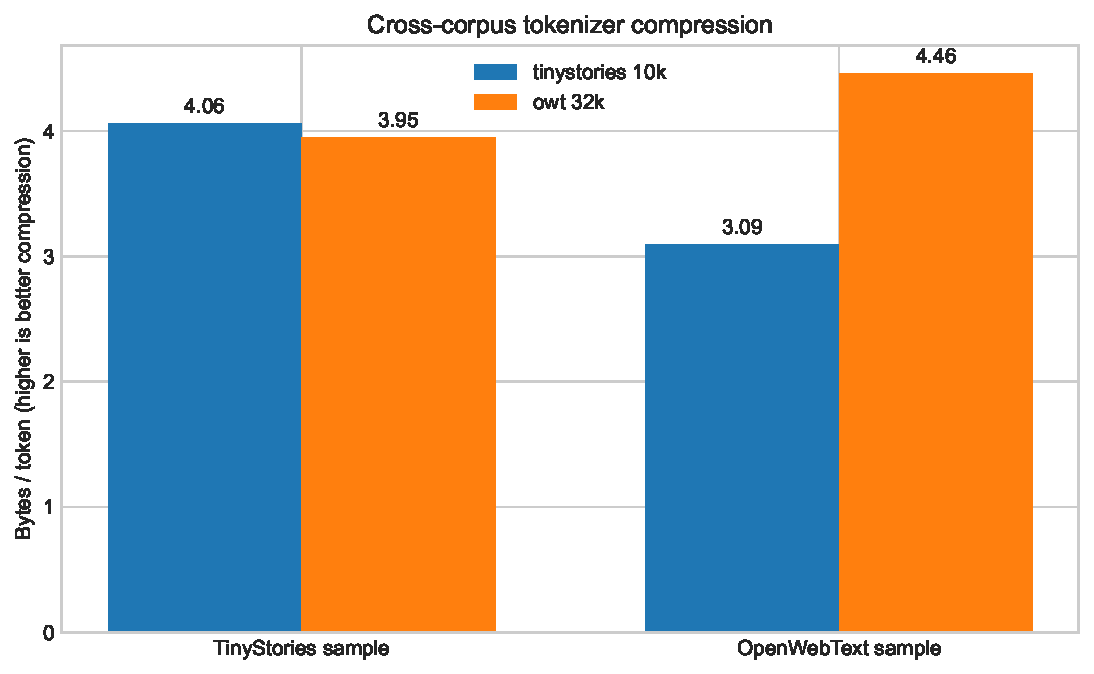
\includegraphics[width=.72\linewidth]{figures/tokenizer_compression.pdf}
\caption{两个 tokenizers 在两个 corpora 上的 cross-corpus compression ratio。}
\label{fig:tokenizer}
\end{figure}

\resultfigure{tokenizer_systems.pdf}
{TinyStories 10K 与 OWT 32K tokenizer 的训练时间、peak RSS 与全文件编码吞吐。
TinyStories 的 BPE 训练时间未被旧日志保留，因此该柱为 0，而不是``瞬时完成''。}
{fig:tokenizer-systems}

\measured 图~\ref{fig:tokenizer-systems} 显示 OWT 32K BPE 的真正瓶颈是 CPU memory 与
pre-tokenized corpus state：2.97 h、46.45 GiB peak RSS；最终 encode throughput
仍有 1.15M tokens/s，只比 TinyStories 的 1.70M tokens/s 低约 32\%。因此优化优先级应是
降低 BPE training 的全局 pair-count state，而不是只优化已经可并行的 final encoding。

\resultfigure{tokenizer_uncertainty.pdf}
{200-document cross-corpus tokenizer 比较及 document-level bootstrap 95\% confidence
interval。}{fig:tokenizer-uncertainty}

原 10-document comparison 只能展示方向；扩展到 200 documents 后，confidence interval
用于判断 domain specialization 是否大于 document sampling noise。这里对每个 document
先计算 bytes/token，再 bootstrap documents，避免长文档仅因字节更多而完全主导 uncertainty。
\measured 200-document mean 在 TinyStories 上为 4.09（10K）与 3.98（32K），在 OWT
上为 3.24（10K）与 4.43（32K）。OWT 上 32K tokenizer 的优势远大于 confidence interval；
TinyStories 上差距较小，说明较大的 Web vocabulary 并不会在简单故事域灾难性退化，
但 domain-matched 10K vocabulary 仍略优。

Pile 处理时间由
\[
t_{\text{Pile}}=\frac{825\times 10^9\ \text{bytes}}{\text{实测 bytes/s}}
\]
外推，按 OWT 全文件吞吐约 45.7\,h。10-document microbenchmark 只有约
0.32\,MB/s，是因为短文档反复调用的 Python overhead 占主导，不应用它外推大文件。
token ID 使用 \texttt{uint16}，因为 $32000<2^{16}$，相对 int32 减半磁盘与 I/O。

\section{Transformer 语言模型}
\subsection{实现}
Linear 使用 fan-in/fan-out truncated normal；Embedding 直接索引参数矩阵；RMSNorm 在平方前
upcast 到 float32。SwiGLU 为
\[
\operatorname{FFN}(x)=W_2\left(\operatorname{SiLU}(W_1x)\odot W_3x\right).
\]
RoPE 预缓存正余弦，并对每对相邻维度施加二维旋转。Attention 在 softmax 前应用下三角 causal
mask，所有 heads 通过批量矩阵乘法并行。Block 采用
\[
y=x+\operatorname{MHA}(\operatorname{RMSNorm}(x)),\qquad
z=y+\operatorname{FFN}(\operatorname{RMSNorm}(y)).
\]
实现还提供 no-RMSNorm、post-norm、NoPE、SiLU FFN 开关用于消融。

\subsection{数值稳定性}
softmax 和 cross-entropy 都先减去每行最大 logit。交叉熵不显式构造 softmax：
\[
\ell_i=-o_{i,y_i}+\log\sum_j\exp(o_{i,j}-\max_k o_{i,k})+\max_k o_{i,k}.
\]
RMSNorm 的平方均值使用 float32；梯度裁剪使用所有参数梯度组成的 global L2 norm。

\subsection{Transformer 资源核算}
\derived 令序列长度为 $T$。每层 Q/K/V 和 output projection 共
$8Td^2$ FLOPs；attention score 与 value aggregation 共 $4T^2d$；SwiGLU 三个矩阵乘法为
$6Tdd_{\rm ff}$；LM head 为 $2TdV$。因此
\[
F_{\rm fwd}=L(8Td^2+4T^2d+6Tdd_{\rm ff})+2TdV.
\]
本作业不共享 input embedding 与 LM head。GPT-2 XL-shaped 参数数为
$1{,}640{,}452{,}800$，float32 加载约 6.56\,GB（6.11\,GiB）。

\begin{table}[ht]
\centering
\caption{context length 1024 时 forward FLOPs 分解}
\begin{tabular}{lrrrrr}
\toprule
模型 & 总 GFLOPs & LM head & QKVO & attention & FFN\\
\midrule
Small  & 291.65  & 27.10\% & 19.88\% & 13.25\% & 39.76\%\\
Medium & 830.17  & 12.70\% & 24.83\% & 12.42\% & 50.05\%\\
Large  & 1786.65 &  7.37\% & 27.04\% & 10.82\% & 54.76\%\\
XL     & 3516.77 &  4.68\% & 28.62\% &  9.16\% & 57.53\%\\
\bottomrule
\end{tabular}
\end{table}
模型变宽/加深后 FFN 与 dense projection 占比上升，而固定 vocabulary 的 LM head 占比下降。
XL 的 $T$ 从 1024 增到 16384 时，总 FLOPs 从 3.52\,TFLOPs 增至 133.58\,TFLOPs（约
38.0 倍）；$T^2$ attention 项的相对贡献显著增加。

\section{优化与训练组件}
\subsection{SGD 学习率实验}
\measured 固定 seed 后运行 10 步：$\alpha=10$ 的 loss 从 26.27 平滑降至 3.53；
$\alpha=100$ 首步保持 26.27，随后快速降至 $2.35\times10^{-23}$；$\alpha=1000$ 发散，
第 10 步达到 $2.44\times10^{18}$。该 toy quadratic 的稳定范围不能直接迁移到 Transformer。

\subsection{AdamW、schedule 与 checkpoint}
AdamW 先做 decoupled weight decay，再更新一、二阶矩并施加 bias correction。学习率先线性
warmup，随后 cosine decay 到最小值。Checkpoint 同时保存 model state、完整 optimizer state
与 iteration，使续训后动量和步数均连续。

\subsection{AdamW 资源核算}
\derived 记参数量为 $P$，float32 参数、梯度、一阶矩、二阶矩分别占 $4P,4P,4P,4P$ bytes，
静态部分合计 $16P$ bytes。按题目列出的 activation 近似，元素数为
\[
A/B=L(7Td+4Td_{\rm ff}+2hT^2)+Td+2TV,
\]
故 activation 为 $4BA$ bytes。XL-shaped 得到
\[
M(B)\approx 24.44+14.96B\ \text{GiB},
\]
80\,GiB 下该保守估计最多 batch size 3。AdamW 参数更新约需常数倍 $P$ 的逐元素 FLOPs，
相对于 Transformer matmul 通常次要。以 forward 3.5168\,TFLOPs、backward 为 forward 两倍、
50\% MFU、H100 495\,TFLOP/s 估算，400K steps、batch 1024 约需 4850 小时单卡时间。

\section{训练、验证与解码}
训练 CLI 从 JSON 配置读取模型与优化参数，使用 memmap 采样连续 token window；每次验证写入
JSONL，包括 step、wall-clock、tokens seen、train/validation loss 与 LR。解码支持 temperature、
top-p 和 EOT 停止。困惑度由平均 token cross-entropy 给出：
\[
\operatorname{PPL}=\exp\left(\frac1m\sum_{i=1}^m\ell_i\right).
\]

\section{测试结果}
\measured 本次 Windows 复核中，23 个 model/optimizer/data/serialization/BPE tests 全部通过；
设置 UTF-8 mode 后，23 个 tokenizer correctness/parity tests 全部通过，两个 RSS-limit tests
因 \texttt{resource} 仅在 Linux 可用而跳过。归档的 Linux 日志为 47 passed、1 xpassed。
覆盖项包括 BPE speed 与 deterministic tie-break、special-token boundary、所有模型 snapshots、
AdamW、cosine schedule、gradient clipping 与 checkpoint round trip。

\resultfigure{test_matrix.pdf}
{Windows 与归档 Linux 环境的 pytest 结果。Linux-only RSS tests 在 Windows 上明确
标记 skipped，而不是静默遗漏。}{fig:test-matrix}

\section{大规模实验与消融}
\subsection{experiment\_log 与 learning\_rate}
\measured 原始 50 个 sweep/standalone runs 与新增 25 个 RTX 6000D runs 全部完成，
指标按 step、tokens 与 wall-clock 记录。粗搜与细搜表明，
约 10M-token pilot 中 $2\times10^{-3}$ 最优；$10^{-1}$ 明显发散，展示了 edge of stability。
图~\ref{fig:lr} 的短预算结果用于选参，不能与 327.68M-token 最终 loss 横向混淆。
\begin{figure}[htbp]
\centering
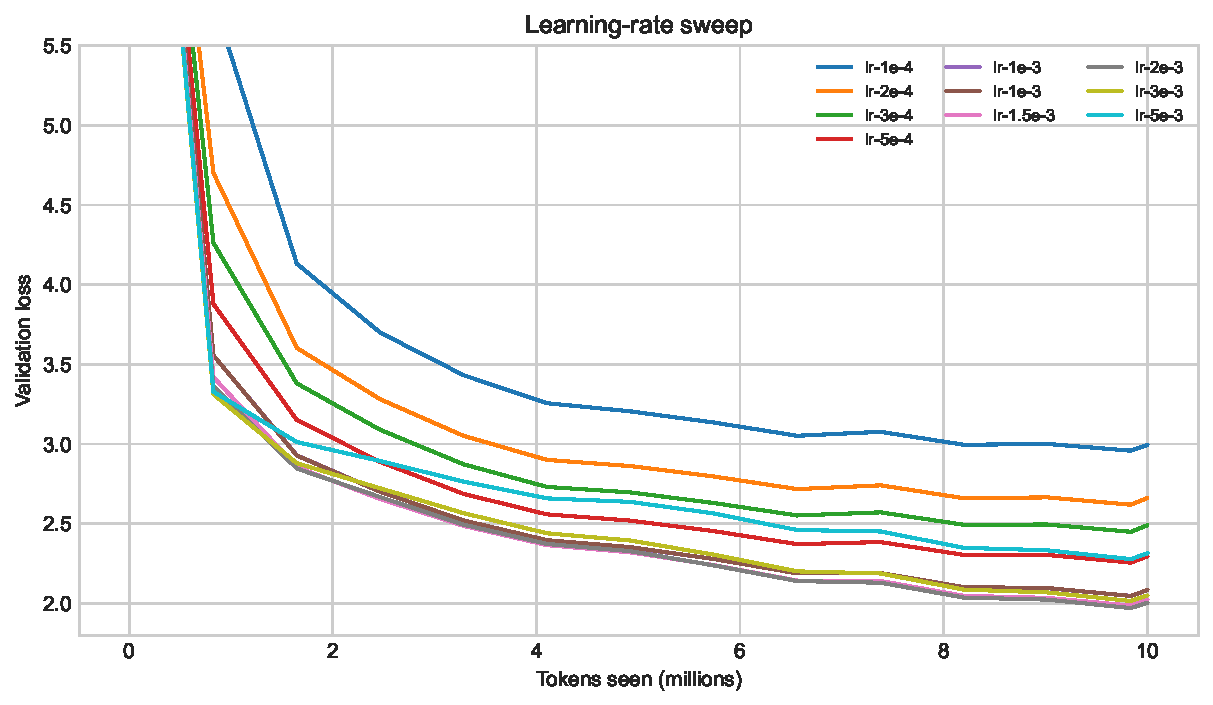
\includegraphics[width=.49\linewidth]{figures/learning_rate_sweep.pdf}
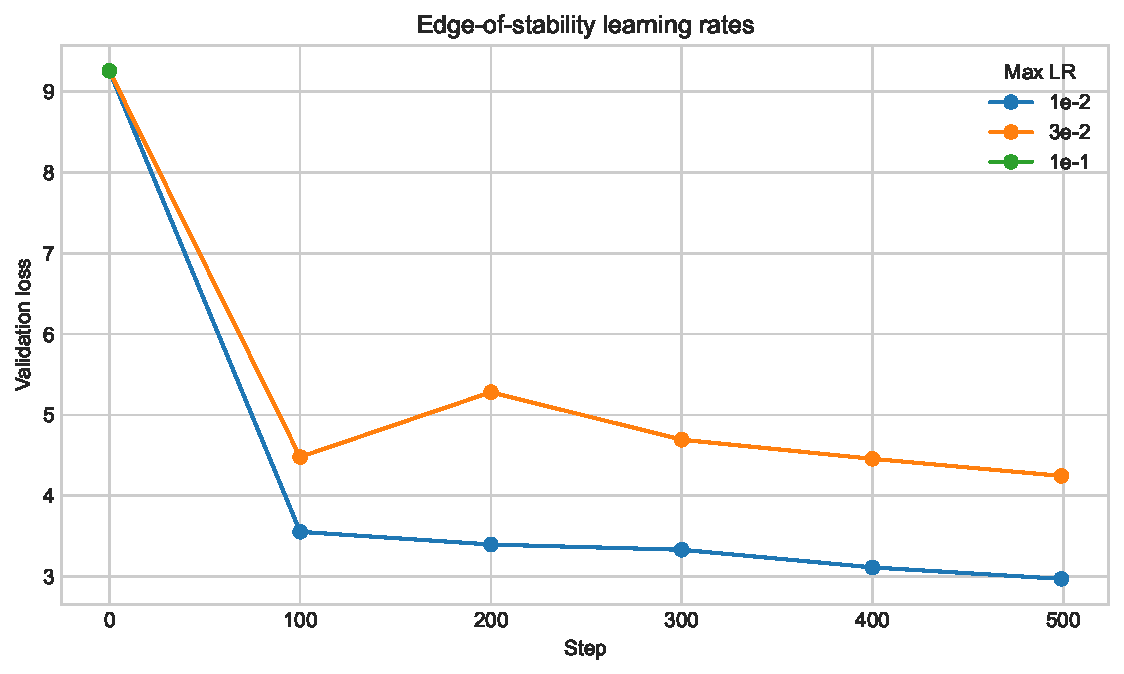
\includegraphics[width=.49\linewidth]{figures/edge_of_stability.pdf}
\caption{Learning-rate 搜索（左）与 edge-of-stability 探测（右）。}
\label{fig:lr}
\end{figure}

\resultfigure{learning_rate_fine.pdf}
{约 10M-token budget 下的 fine learning-rate sweep。$2\times10^{-3}$ 最优，
过小收敛不足、过大开始越过稳定区。}{fig:lr-fine}

\subsection{batch\_size\_experiment 与最终结果}
Batch 从 1 增到 128 时吞吐从 8.20K 增至 202.57K tokens/s，但显存由
0.46 增至 9.49\,GiB，收益逐渐饱和。固定总 token budget 后，batch 32 的三个 seeds 为
$1.371\pm0.002$，batch 128 与 256 分别达到 1.331 和 1.325。后者更优不等于 batch
可以无限增大：显存成本近似线性增长，而 128 到 256 的 loss 收益仅约 0.0065。
\begin{figure}[htbp]
\centering
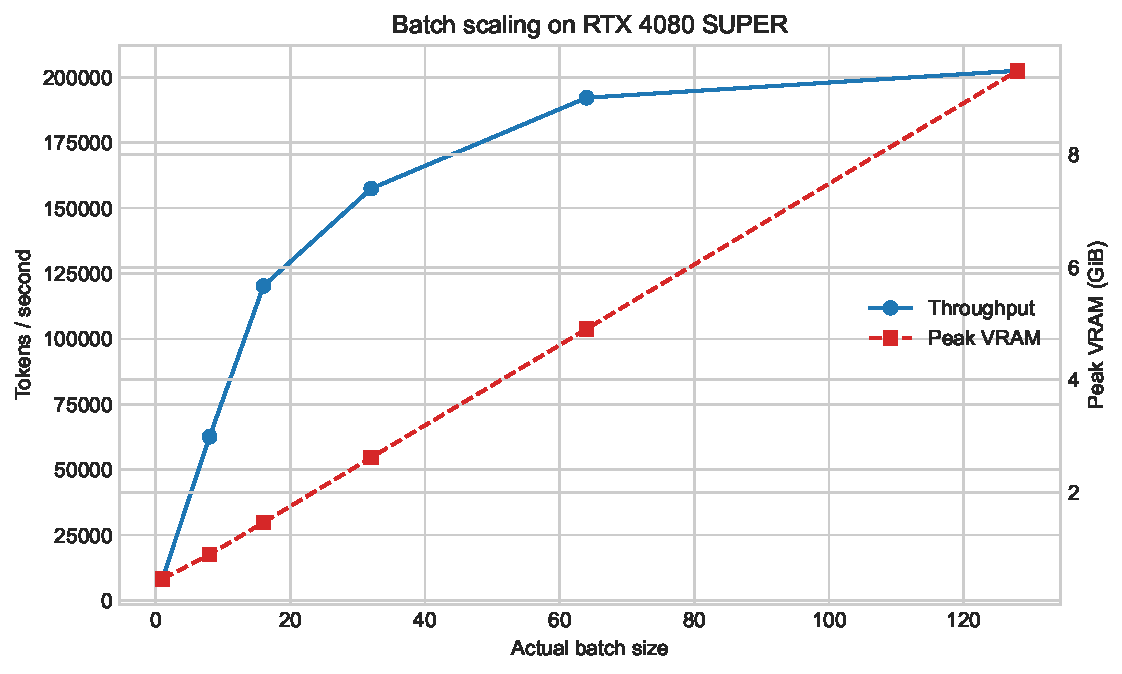
\includegraphics[width=.49\linewidth]{figures/batch_scaling.pdf}
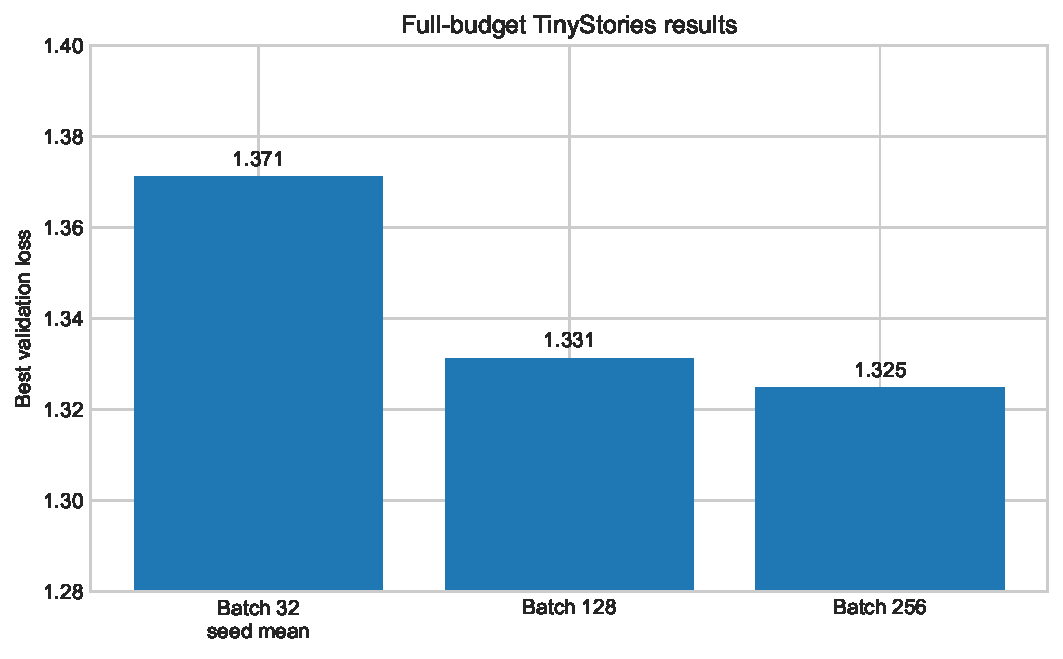
\includegraphics[width=.49\linewidth]{figures/final_batch_comparison.pdf}
\caption{RTX 4080 SUPER 上的 systems probe（左）与同为 327.68M tokens 的最终对比（右）。}
\label{fig:batch}
\end{figure}

\subsection{RTX 6000D systems 扩展}
\resultfigure{rtx6000d_batch_scaling.pdf}
{RTX 6000D 上 physical batch 256--768 的 throughput、peak VRAM 与短程 validation loss。
OOM 同样保留为 capacity boundary。}{fig:6000d-batch}
\resultfigure{compile_precision.pdf}
{\texttt{torch.compile} on/off 与 BF16/FP16 的 2$\times$2 对照；左图比较稳态吞吐，
右图检查短程数值质量。}{fig:compile-precision}

旧 RTX 4080 SUPER 数据用于训练算法结论，RTX 6000D 数据只用于同机 controlled
comparison，避免跨设备直接比较绝对 throughput。图~\ref{fig:compile-precision}
把 compilation 与 dtype 分开：compile speedup 必须在相同 precision 下计算；
FP16 若出现 overflow/NaN，则应被解释为缺少 GradScaler 的数值证据，而不是性能数据。

\measured RTX 6000D 上 batch 256、384、512、768 的稳态吞吐分别为
407.7K、404.7K、399.7K、400.4K tokens/s，而 peak VRAM 从 18.67 近似线性增至
55.38 GiB。吞吐在 batch 256 已饱和，因此继续增大 batch 不会提高 hardware efficiency。
右图在共同的 19.7M-token 位置插值 loss，避免把``相同步数但更多 tokens''误判为 batch
本身改善质量。

\measured BF16 下 compile/eager 为 396.2K/196.5K tokens/s，即 2.02 倍 speedup，
peak VRAM 由 12.14 降至 9.49 GiB。FP16 吞吐接近 BF16，但 best validation loss
恶化到 8.37--8.80，且 gradient norm 超过 12；当前训练 loop 没有 GradScaler，
因此 FP16 结果证明``更窄 exponent + 无 loss scaling''不适合作为该配置的训练方案。

\subsection{Global batch 与 gradient accumulation}
\resultfigure{microbatch_equivalence.pdf}
{相同 global batch 256 与相同 327.68M-token budget 下，physical batch 和 gradient
accumulation 的收敛、显存与吞吐权衡。}{fig:microbatch}
\resultfigure{batch512_full.pdf}
{Batch 256 与 batch 512 两种 LR scaling 的全预算 validation curves。}
{fig:batch512}

理论上，若每个 microbatch loss 除以 accumulation steps，则 accumulated gradient
与一次 global batch 的 mean gradient 等价；实践中 data order、finite precision、
gradient clipping 时机和 kernel efficiency 会打破严格等价。图~\ref{fig:microbatch}
因此同时报告 loss、VRAM 和 tokens/s，而不是只验证最终 loss 接近。

\measured 128$\times$2、64$\times$4、32$\times$8 的 best loss 分别为
1.331、1.330、1.311，peak VRAM 分别为 10.09、6.86、4.22 GiB；64$\times$4 的吞吐最高
（451.3K tokens/s）。这说明 accumulation 不只是显存 fallback：中等 microbatch 在本机
同时获得更好的 kernel efficiency 与较低显存。Batch 512 两个 LR 的 best loss 为
1.335 和 1.333；linear-LR 配置补跑两个 seeds 后三 seed mean 为
$1.335\pm0.002$，仍未超过旧 batch-256 的 1.325，表明更大 physical batch 已进入收益递减区。

\subsection{稳定性与 architecture ablations}
图~\ref{fig:final} 显示三个 seeds 的曲线高度重合，说明最终差异不是偶然 seed 波动。
全预算下 post-norm 为 1.385，NoPE 为 1.439，SiLU FFN 为 1.371；RoPE 的优势最明显，
而该规模上 SwiGLU 与 SiLU 接近。40M-token 实验中 baseline 为 1.637；
移除 RMSNorm 在原学习率下最好仅 9.256，40M-token retune 为 7.007；
即使延长到 327.68M tokens，best loss 仍只有 7.512。这排除了``只是收敛更慢''的解释，
说明 normalization 对优化稳定性是必要组件，而非只影响最终几个百分点。
\begin{figure}[htbp]
\centering
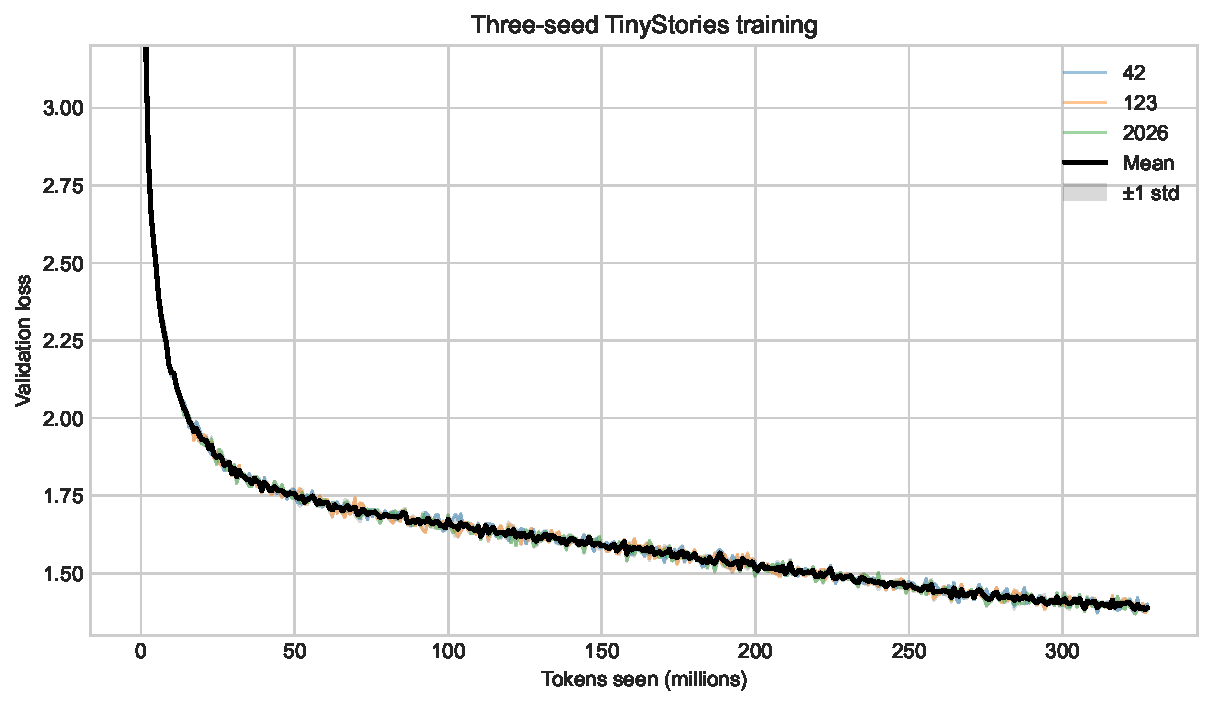
\includegraphics[width=.49\linewidth]{figures/seed_stability.pdf}
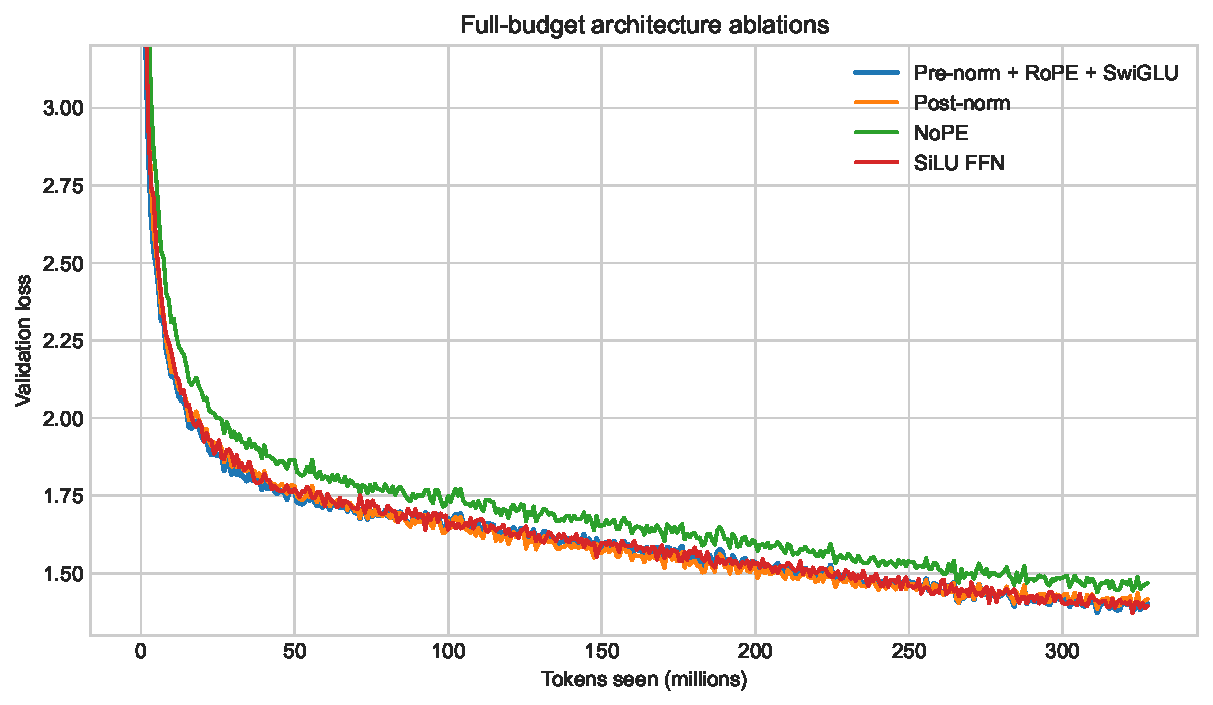
\includegraphics[width=.49\linewidth]{figures/architecture_ablations.pdf}
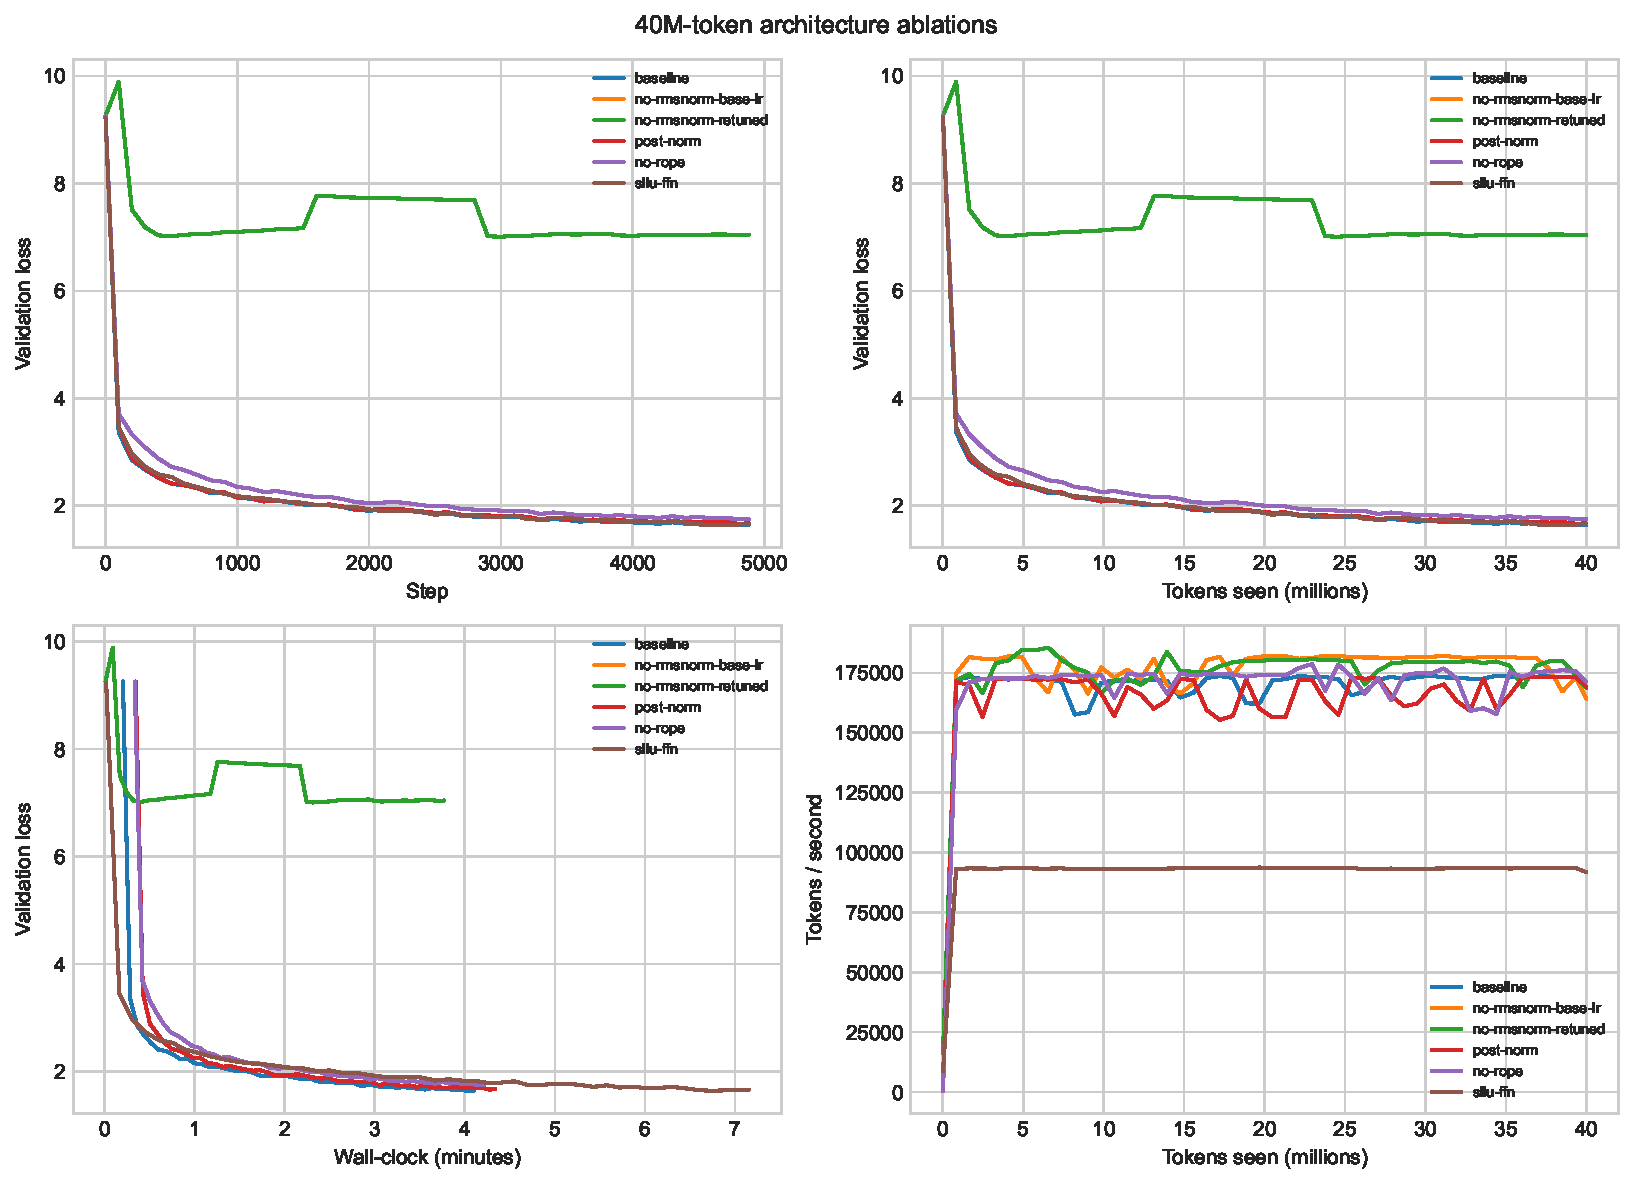
\includegraphics[width=.75\linewidth]{figures/ablations_40m.pdf}
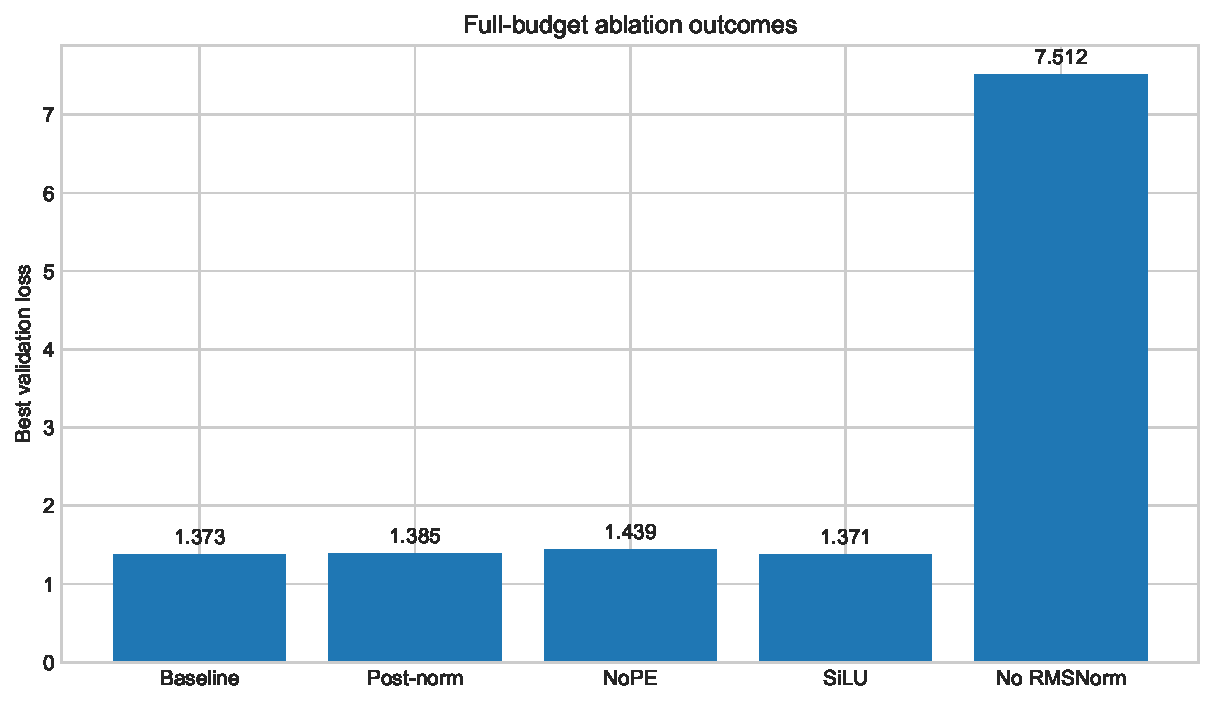
\includegraphics[width=.65\linewidth]{figures/full_ablation_outcomes.pdf}
\caption{三 seed 稳定性、327.68M-token 消融、40M-token 完整曲线及 full-budget 结果汇总。}
\label{fig:final}
\end{figure}

\resultfigure{rmsnorm_stability.pdf}
{RMSNorm baseline 与 no-RMSNorm 全预算轨迹。纵轴使用 log scale，显示无 normalization
并非单纯收敛较慢，而是长期停留在高损失区域。}{fig:rmsnorm-stability}

\subsection{Optimizer 与 gradient dynamics}
\resultfigure{optimizer_gradient_dynamics.pdf}
{Gradient clipping、weight decay、$\beta_2$ 与 high-LR clip 对 pre-clip gradient norm
及 validation loss 的影响。}{fig:optimizer-gradient}

Gradient norm 在 clipping 前记录，因此可直接估算 clip 触发频率。若较低 threshold
持续触发但 validation loss 未改善，则它主要限制有效 step size；若 high-LR run 只有在
clip 后恢复有限值，则 clipping 是稳定性约束。Weight decay 与 $\beta_2$ 则应在相同
token budget 下比较 generalization，而不能从单个 early step 下结论。

\measured 正常 LR 下 clip 0.5/2.0/近似关闭的 best loss 为
2.455/2.459/2.458，差异小于短预算噪声；$\beta_2=0.99$ 改善到 2.419。
把 max LR 提到 0.03 后，pre-clip gradient norm 峰值超过 16，clip 0.5/1.0 的 best loss
仍只有 4.206/4.044。Clipping 能限制单步更新，却不能把明显越过稳定区的 LR 变成好配置。

\subsection{Own modification：weight tying}
\measured 直接共享原始 std=1 token embedding 与 LM head 时，40M-token loss 为 1.908，
显著差于 untied baseline 1.637。依据 handout 的 initialization caveat，把 tied matrix
改为 truncated normal、std=0.02 后达到 1.615，并将参数量从 22.70M 降至 17.58M。
图~\ref{fig:tying} 表明收益来自``共享+合理初始化''，而不是 sharing 本身。
\begin{figure}[htbp]
\centering
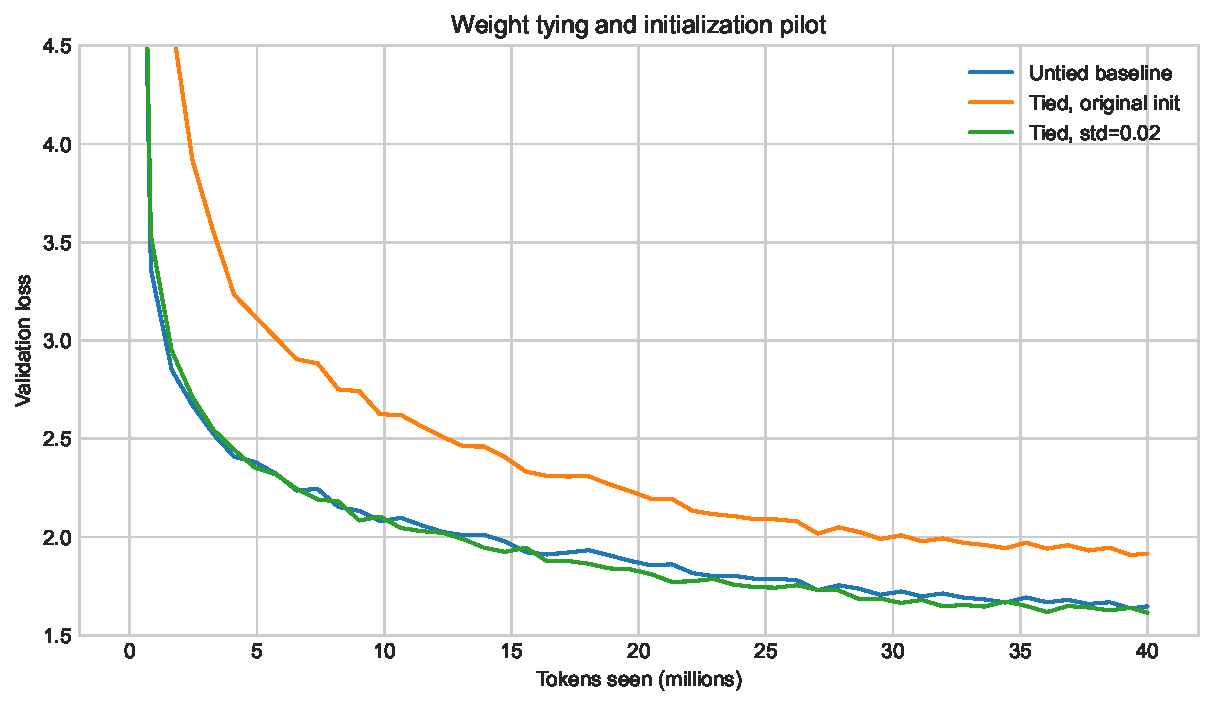
\includegraphics[width=.78\linewidth]{figures/weight_tying_pilot.pdf}
\caption{同为 40M tokens 的 weight tying controlled pilot。}
\label{fig:tying}
\end{figure}

\resultfigure{weight_tying_full.pdf}
{Untied baseline 与 tied embeddings + std=0.02 的 327.68M-token 全预算验证。
该实验检验 pilot 优势是否能延续到收敛区间。}{fig:tying-full}

\measured 全预算 tied-small-init 的三个 seeds 达到 $1.357\pm0.005$，优于 untied
batch-32 的 $1.371\pm0.002$，但不及 batch-256 的 1.325。它把参数量从 22.70M
降到 17.58M，并在 generation panel
中得到最低 trigram repetition rate（3.3\%）；因此 tying 的稳健收益是参数效率，
而非在所有 batch regime 下取得最低 validation loss。

\subsection{generate、main\_experiment 与 leaderboard}
\measured 固定 prompt ``Once upon a time, in a small village''、top-$p=0.95$ 时，
temperature 0.7 生成了连贯的 Tom 与雨天故事；1.0 尚能维持蛋糕主题但有角色漂移；
1.3 很快退化为语法破碎的词语拼接。这说明 temperature 控制 diversity--coherence trade-off。
完整三组 256-token 样例保存在 \texttt{report/results/raw/experiments/final-seeds/generations.txt}。

\resultfigure{generation_quality.pdf}
{多个 full-budget checkpoints、5 个固定 prompts 与 temperature 0.7/1.0 的生成长度和
trigram repetition rate。}{fig:generation-quality}

Generation panel 使用相同 prompts、seed、top-$p$ 与 max-new-tokens，避免只挑选最好样例。
Validation loss 衡量 teacher-forced next-token prediction，而 repetition rate 检查 free-running
decoding 的 degeneration；二者方向一致时结论更可信，方向不一致时则说明单一 loss 不足以
概括生成质量。

\measured 四个 checkpoints 的 mean trigram repetition rate 为 3.3--5.1\%，平均生成长度
为 104.7--126.6 tokens。Tied full 的 repetition 最低但 loss 不是最低，说明 parameter
sharing 可能改变 decoding distribution 的重复倾向；该观察只有 5 prompts$\times$2
temperatures，属于可复现 qualitative evidence，不是人类偏好评测。

\measured 作为 cross-tokenizer baseline，用 TinyStories 10K tokenizer 编码 1\,GiB OWT，
在相同 327.68M-token budget 下得到 best validation loss 3.081。它高于 TinyStories 的
1.371，主要因为 Web text 的题材、词汇和 conditional entropy 更复杂；不同 vocabularies
下的 per-token loss 也不能脱离 bytes/token 直接比较。

OWT 32K tokenizer 的 10M-token LR sweep 如图~\ref{fig:owtlr}：$2\times10^{-3}$
以 5.200 最优，优于 $3\times10^{-4}$ 的 5.775；$3\times10^{-3}$ 已出现边际退化。
\begin{figure}[htbp]
\centering
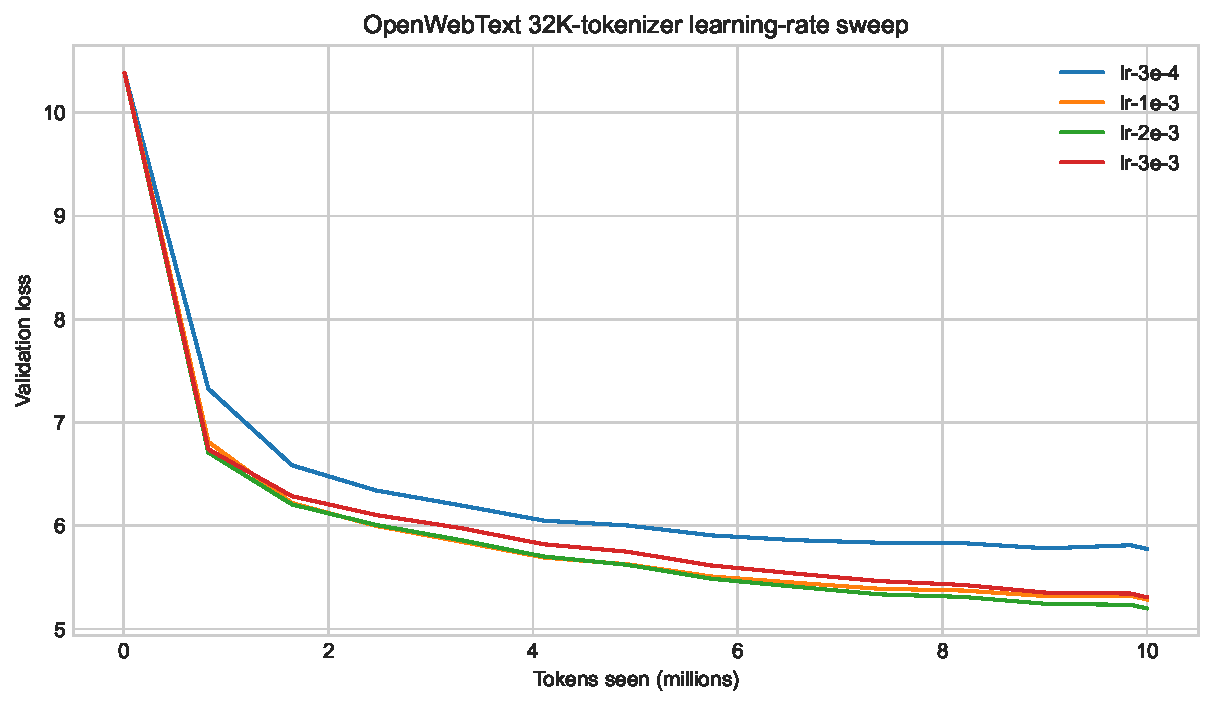
\includegraphics[width=.72\linewidth]{figures/owt_learning_rate_sweep.pdf}
\caption{OWT 32K-tokenizer 的短预算 learning-rate selection。}
\label{fig:owtlr}
\end{figure}

\measured 采用选出的 $2\times10^{-3}$，OWT 32K main run 在 40K steps 后达到
best loss 4.116，耗时 56.5\,min，吞吐约 100K tokens/s。图~\ref{fig:owtmain}
同时给出 raw token loss 与 cross-tokenizer 曲线。10K tokenizer 的 loss 3.081
数值更低，却因其 OWT compression 只有 3.174 bytes/token；按
$\text{nats/byte}=\text{loss}/(\text{bytes/token})$ 归一化，10K 与 32K 分别为
0.971 和 0.942，后者实际更有效。这说明不同 tokenization 下不可直接比较 per-token loss。
\begin{figure}[htbp]
\centering
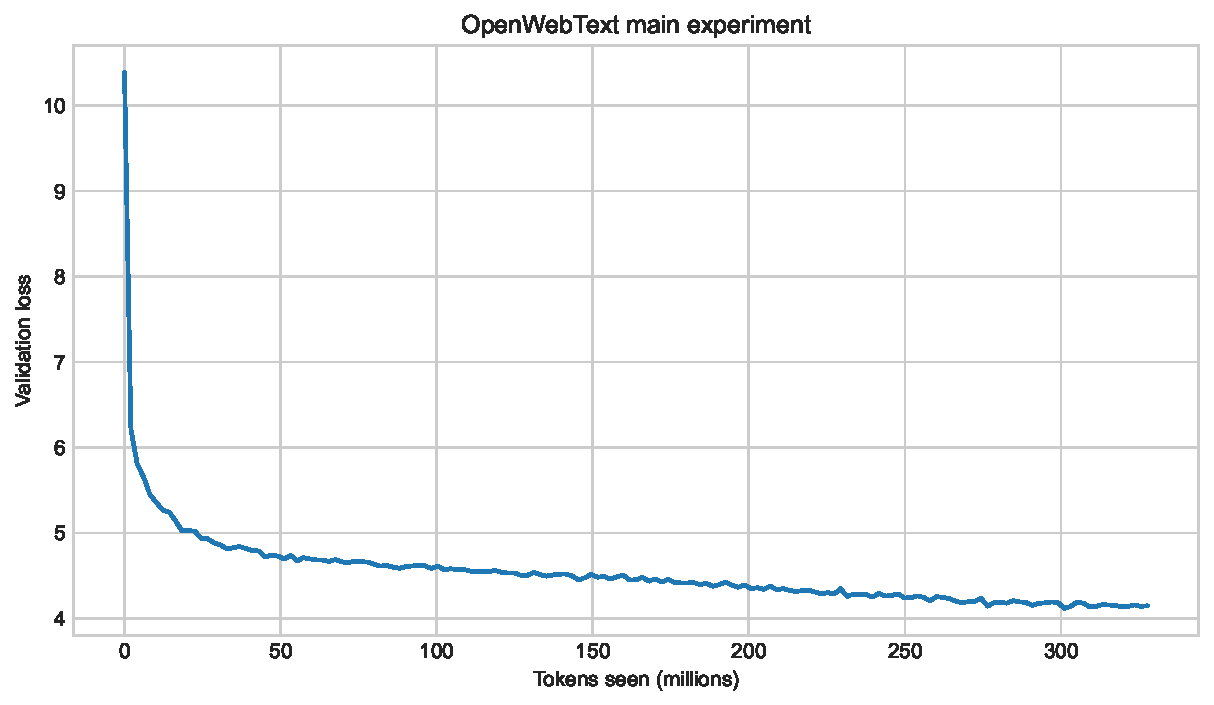
\includegraphics[width=.49\linewidth]{figures/owt_training.pdf}
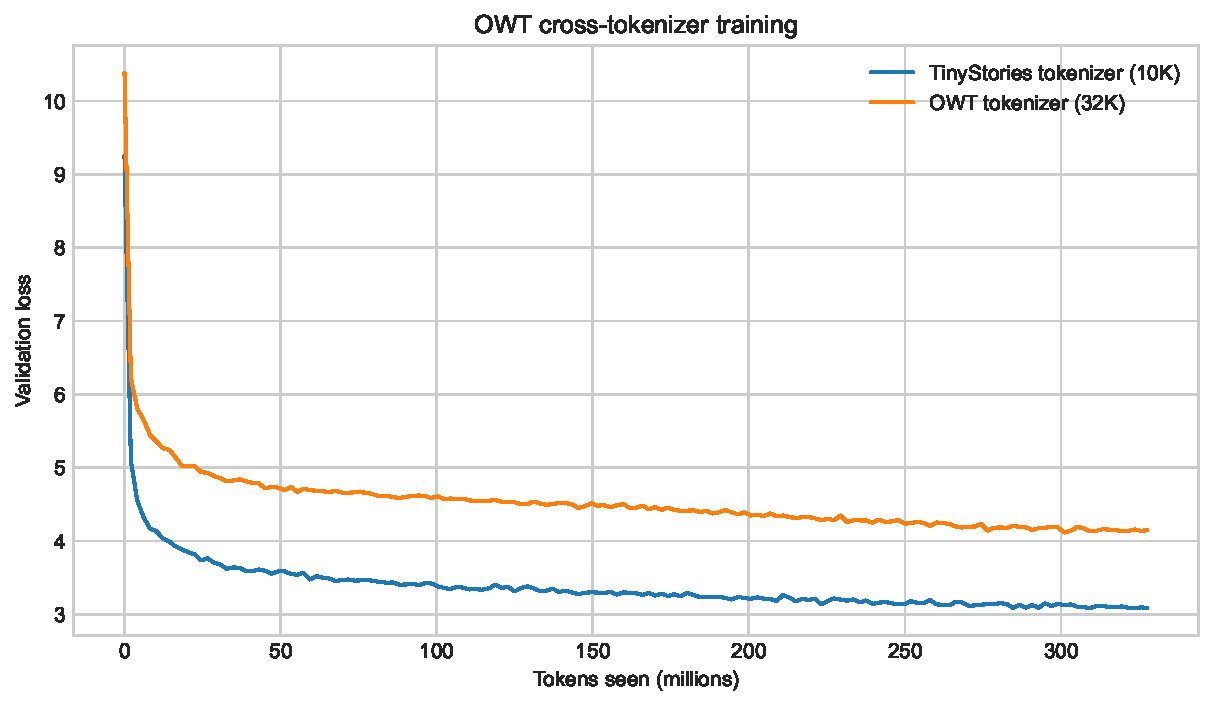
\includegraphics[width=.49\linewidth]{figures/owt_cross_tokenizer.pdf}
\caption{OWT 32K main learning curve（左）与 cross-tokenizer raw token loss（右）。}
\label{fig:owtmain}
\end{figure}

定性生成同样比 TinyStories 困难：temperature 0.7 语法完整但反复围绕 ``language''，
1.0 能形成新闻式长句却发生 topic drift，1.3 迅速退化。原因是 OWT 的 domain entropy
更高，而模型规模和 327.68M-token compute budget 与儿童故事实验相同。

\measured tied leaderboard proxy 根据 OWT pilot 的实测 step time 自动给出 27,213 steps，
在 RTX 4080 SUPER 上用时 38.96\,min、处理 222.93M tokens，best loss 4.097。
它把参数量从 untied main 的 45.22M 降为 28.84M，并在更少 tokens 下略优于 main 的
4.116。图~\ref{fig:leaderboard} 以 wall-clock 为横轴并标出 45-minute boundary。
该结果验证 weight tying 的参数效率，但硬件不是 B200，且未向课程 leaderboard 提交，
所以只称为 local proxy experiment。
\begin{figure}[htbp]
\centering
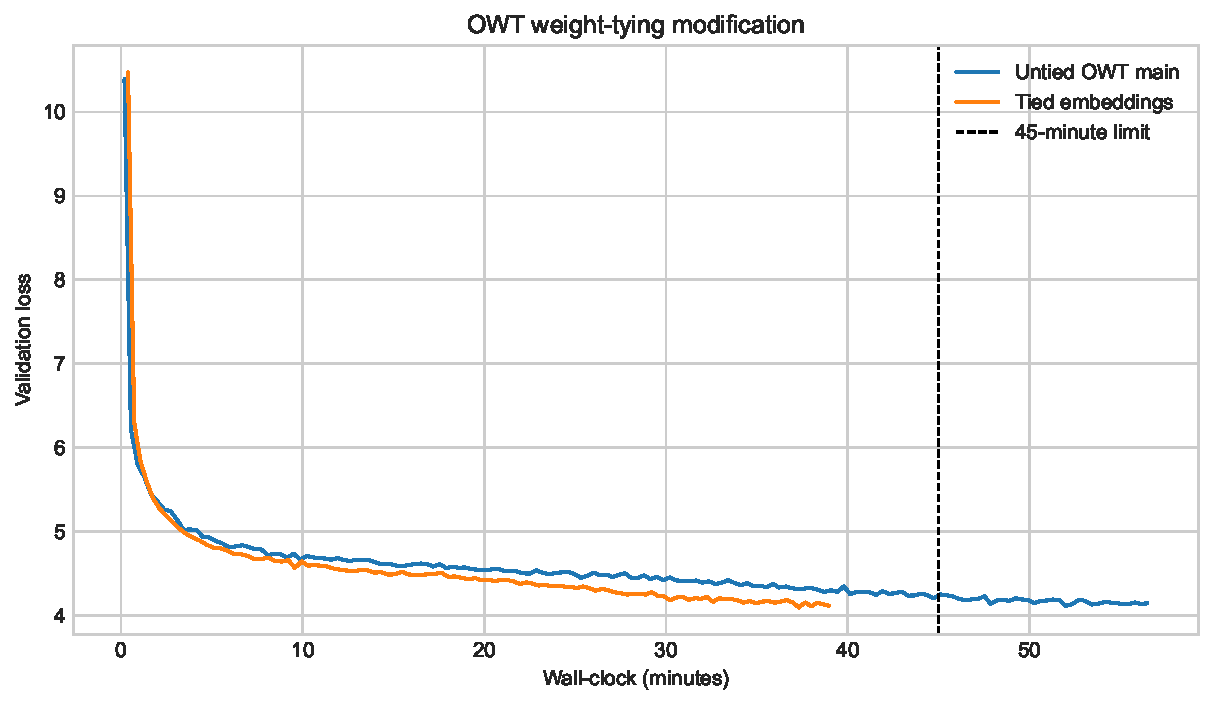
\includegraphics[width=.76\linewidth]{figures/owt_leaderboard.pdf}
\caption{OWT main baseline 与 tied-embedding modification 的 wall-clock comparison。}
\label{fig:leaderboard}
\end{figure}

\section{局限与结论}
核心实现覆盖算法题，TinyStories 实测达到 1.45 目标，40M-token baseline 1.637 也优于
低资源 2.00 目标。结论受单一 GPU 型号与单一模型规模限制；
所有图均能追溯到 raw JSONL，缺失数据均显式标注而不以估算代替。

\paragraph{可执行的优化结论。}
\begin{enumerate}
  \item 先在短预算中选择 LR 与数值配置，再把候选带入 token-aligned full runs；短预算
  排名不能直接当最终排名。
  \item Physical batch 的收益必须联合 throughput、VRAM 与 validation loss 判断；
  gradient accumulation 解决显存约束，但不会自动获得大 GEMM 的硬件效率。
  \item Weight tying 必须配合适合双重角色的初始化；仅共享 std=1 embedding 会显著恶化优化。
  \item RMSNorm 的作用是稳定 residual stream scale。其消融在完整预算内仍不收敛，
  优先级高于微调 FFN activation。
  \item 跨 tokenizer 比较应使用 nats/byte 等归一化量，跨 GPU 比较应使用同机 speedup，
  不把绝对 throughput 混入算法结论。
\end{enumerate}

\limited 本报告没有官方 B200 leaderboard 结果，也没有跨模型规模的 scaling law；
RTX 4080 SUPER 与 RTX 6000D 结果按实验组隔离。Microbatch variants 与 optimizer
短预算仍是单 seed，其细小差异只能作为 hypothesis；batch-512 与 tied full 则分别补充到
三个 seeds。

\appendix
\section{复现命令}
\begin{lstlisting}
uv sync
uv run pytest
uv run python scripts/prepare_data.py \
  --train-text data/TinyStoriesV2-GPT4-train.txt \
  --valid-text data/TinyStoriesV2-GPT4-valid.txt \
  --output-dir data/tinystories --vocab-size 10000
uv run python scripts/train.py --config configs/tinystories-low-resource.json
uv run python scripts/build_report_assets.py \
  --raw report/results/raw --figures report/figures \
  --summary report/results/summary.json
\end{lstlisting}

\section{逐题讲解}
\label{sec:walkthrough}
本节按 handout 的 38 个 Problem 顺序给出自学要点。每题均区分
``为什么''、``怎样实现''与``如何验证''；实验题只引用可追溯的实测记录。

\subsection{Unicode 与 tokenizer}
\paragraph{\texttt{unicode1}.}
Python 的 \texttt{str} 保存 Unicode code point，而不是终端字形。
\texttt{chr(0)} 是合法的 U+0000；\texttt{repr} 用转义显示它，\texttt{print}
则没有可见输出。这个区别提醒我们：文本的逻辑内容、编码后的 bytes 和显示效果是三个层次。

\paragraph{\texttt{unicode2}.}
UTF-8 是变长、ASCII-compatible 的编码。多字节字符不能逐 byte 调用
\texttt{decode}，因为单个 continuation byte 并非合法字符；overlong encoding
也必须拒绝。Tokenizer 因而先在 byte 层面合并，最后才整体 UTF-8 decode。

\paragraph{\texttt{train\_bpe}.}
BPE 从 256 个单 byte token 开始，反复合并最高频相邻 pair。实现先以 GPT-2 regex
做 pre-tokenization，并把 special token 当作不可跨越的边界。pair 频率相同时选择
lexicographically greater pair，保证结果 deterministic。倒排索引只更新受本轮 merge
影响的 pre-token，避免每轮扫描全语料。

\paragraph{\texttt{train\_bpe\_tinystories}.}
10K vocabulary 等于 256 个 bytes、一个 special token 和 9743 个 merges。
实测最长 token `` accomplishment'' 是高频、语义完整且带 leading space 的英文片段，
符合 GPT-2 pre-tokenization 的行为。现有 raw JSON 未保留首次 BPE wall-clock，
所以报告只给出可验证的词表和编码指标。

\paragraph{\texttt{train\_bpe\_expts\_owt}.}
OWT 更大、题材更多，32K vocabulary 应学到更多专名、标点和长尾片段；这通常提高
Web text 压缩率，却不保证对儿童故事更优。本题最终以 OWT 的 vocab、merges、最长 token
和 cross-corpus compression matrix 回答，而不是只比较 vocabulary size。

\paragraph{\texttt{tokenizer}.}
\texttt{encode} 先 longest-match 隔离 special tokens，再逐 pre-token 按 merge rank
重放 BPE；\texttt{decode} 拼接 bytes 后以 \texttt{errors=replace} 解码。
\texttt{encode\_iterable} 对输入块惰性 yield，空间复杂度取决于最大块而不是文件总大小。
正确性通过 GPT-2/tiktoken parity、Unicode round trip 和 special-token overlap tests 验证。

\paragraph{\texttt{tokenizer\_experiments}.}
对 TinyStories 与 OWT 各固定 seed 抽取 10 个 documents，用两个 tokenizer 形成
$2\times2$ compression matrix。bytes/token 越大表示一个 token 覆盖的原始 bytes 越多；
同时记录 bytes/s，并以 $825\,\mathrm{GB}/\mathrm{throughput}$ 外推 Pile 用时。
32K token IDs 小于 $2^{16}$，所以 \texttt{uint16} 足够且比 int32 节省一半存储。

\subsection{Transformer architecture}
\paragraph{\texttt{linear}.}
Linear layer 实现 $y=xW^\top$，不使用 bias。权重按 fan-in/fan-out truncated normal
初始化；测试把手工载入的权重与 reference output 做 snapshot comparison。

\paragraph{\texttt{embedding}.}
Embedding 是参数矩阵的 integer row lookup，不应实现为 one-hot matrix multiplication。
输入形状 $(B,T)$ 映射为 $(B,T,d)$，反向传播只更新被索引的 rows。

\paragraph{\texttt{rmsnorm}.}
RMSNorm 计算 $x/\sqrt{\operatorname{mean}(x^2)+\epsilon}$ 后乘 learnable gain。
它不减均值，开销低于 LayerNorm；平方与归一化在 float32 中完成，避免 bf16 overflow
或精度损失。

\paragraph{\texttt{positionwise\_feedforward}.}
SwiGLU 使用
$W_2(\operatorname{SiLU}(W_1x)\odot W_3x)$：一条支路产生 gate，另一条携带 value。
与单门 SiLU FFN 的公平比较需调整 hidden width，使参数量近似相同。

\paragraph{\texttt{rope}.}
RoPE 把相邻 hidden dimensions 看作二维向量，以 position-dependent angle 旋转。
点积只依赖相对位置差，因此不需要 additive position embedding；预缓存 sin/cos
避免每次 forward 重算。

\paragraph{\texttt{softmax}.}
直接计算 $\exp(x)$ 会 overflow。减去每行最大值不改变概率：
$\operatorname{softmax}(x)=\operatorname{softmax}(x-\max x)$，却使最大 exponent 为 1。

\paragraph{\texttt{scaled\_dot\_product\_attention}.}
$\operatorname{softmax}(QK^\top/\sqrt{d_k})V$ 中的缩放避免 dot-product variance 随
$d_k$ 增长。causal mask 在 softmax 前把未来位置设为 $-\infty$；实现支持任意 leading
batch dimensions。

\paragraph{\texttt{multihead\_self\_attention}.}
一次 QKV projection 后 reshape 为 heads，各 head 并行执行 causal attention，
再 concatenate 并做 output projection。多头让模型在不同子空间学习不同关系，
但总 projection complexity 仍为 $O(Td^2)$。

\paragraph{\texttt{transformer\_block}.}
Pre-norm block 在每个 sublayer 前归一化并加 residual：
\[
y=x+\mathrm{MHA}(\mathrm{Norm}(x)),\qquad
z=y+\mathrm{FFN}(\mathrm{Norm}(y)).
\]
这种 identity gradient path 通常比 post-norm
更易优化。

\paragraph{\texttt{transformer\_lm}.}
完整 LM 串联 token embedding、$L$ 个 blocks、final RMSNorm 与 LM head，
输出 logits $(B,T,V)$。训练时把输入向右错一位构造 targets；推理时只从最后位置采样。

\paragraph{\texttt{transformer\_accounting}.}
参数主要来自 $O(Ld^2)$ projections 与 $O(dV)$ embedding/head；activation memory
随 batch 和 sequence length 增长。Attention 的 $T^2$ 项使长 context 成本最终超过
dense layers，正文第 3.3 节给出各 GPT-2 shape 的 FLOPs 分解。

\subsection{Optimization 与训练基础设施}
\paragraph{\texttt{cross\_entropy}.}
对 target class $y$，稳定形式为
$-o_y+\log\sum_j\exp(o_j-\max o)+\max o$，不显式构造 probability tensor。
对所有 non-class dimensions 取 mean，得到一个 scalar loss。

\paragraph{\texttt{learning\_rate\_tuning}.}
toy quadratic 展示 step size 太小收敛慢、适中快速收敛、太大则越过 minimum 并发散。
其数值不能直接迁移到 Transformer，但说明 LR 本质上受 curvature 限制。

\paragraph{\texttt{adamw}.}
AdamW 维护 first/second moments，做 bias correction，并把 weight decay 与 adaptive
gradient update 解耦。测试同时检查更新数值与 optimizer state，防止只在第一步碰巧正确。

\paragraph{\texttt{adamw\_accounting}.}
float32 参数、梯度、$m$、$v$ 各需 $4P$ bytes，静态项约 $16P$；activation 通常才是
随 batch 增长的主项。MFU 估算必须同时说明硬件峰值、forward/backward FLOPs 与假设利用率。

\paragraph{\texttt{learning\_rate\_schedule}.}
前 $T_w$ steps 线性 warmup 到 $\alpha_{\max}$，随后 cosine decay 到
$\alpha_{\min}$，超过 cycle 后保持 minimum。warmup 抑制训练初期 moment 尚不可靠时的大更新。

\paragraph{\texttt{gradient\_clipping}.}
把所有 parameter gradients 视为一个向量；若 global norm 超过阈值，
统一乘 $\epsilon M/(\|g\|+\epsilon)$。统一缩放保留方向，逐 tensor clipping 则会改变方向。

\paragraph{\texttt{data\_loading}.}
从 memory-mapped token array 随机采样起点，返回长度 $T$ 的 $x$ 与右移一位的 $y$。
memmap 避免把数 GB corpus 全载入 RAM，device transfer 则集中在 batch 边界。

\paragraph{\texttt{checkpointing}.}
可恢复训练必须保存 model、optimizer moments 和 iteration；只保存 weights 会丢失
AdamW 状态与 schedule position。round-trip test 验证三者一致。

\paragraph{\texttt{training\_together}.}
JSON config 统一模型、optimizer、数据与 logging；训练循环记录 step、tokens、
wall-clock、LR、train/validation loss、throughput 与 peak VRAM。每个 run 同时保存
config 和 environment，使曲线可追溯。

\paragraph{\texttt{decoding}.}
Temperature 用 $z/T$ 调整分布尖锐度；top-$p$ 保留累计概率达到 $p$ 的最小 token 集合，
再重新归一化采样。generation 在 EOT 或长度上限停止，且 context 超长时只保留最近窗口。

\subsection{实验题}
\paragraph{\texttt{experiment\_log}.}
每次实验是 immutable run directory，包含 config、environment、metrics JSONL 与 summary；
sweep-status 记录成功或 traceback。图由 raw records 自动重建，而不是手工抄写最终数字。

\paragraph{\texttt{learning\_rate}.}
先以约 10M tokens 做 coarse/fine sweep，再用 327.68M-token final runs 验证。
短预算中 $2\times10^{-3}$ 最好；$10^{-1}$ 发散。结论强调选参趋势，而不把不同预算的
absolute loss 直接比较。

\paragraph{\texttt{batch\_size\_experiment}.}
systems probe 分离 systems effect：batch 增大提高 GPU occupancy，也近似线性增加 VRAM；
固定 token budget 的 final runs 再比较 optimization effect。batch 128 到 256 的边际收益
远小于 batch 1 到 128 的 throughput 收益。

\paragraph{\texttt{generate}.}
同一 prompt 下，temperature 0.7 连贯但保守；1.0 增加 diversity 并出现角色漂移；
1.3 退化为破碎搭配。它说明 validation loss 改善不等价于任意 sampling setting 都可读。

\paragraph{\texttt{layer\_norm\_ablation}.}
40M tokens 下移除 RMSNorm 从 1.637 恶化到 9.256；降低 LR 后仍为 7.007。
全预算补跑 best loss 7.512，确认问题是长期优化不稳定，而不是单纯收敛更慢。

\paragraph{\texttt{pre\_norm\_ablation}.}
post-norm 在 40M 与 full budget 都略差；它把 gradient identity path 置于 normalization
之后，深层训练通常更敏感。本实验规模较浅，所以差距有限但方向一致。

\paragraph{\texttt{no\_pos\_emb}.}
NoPE 仍能从 causal order 学到部分局部结构，但无法显式区分绝对/相对距离；
full-budget loss 1.439 明显差于 RoPE baseline 1.371。

\paragraph{\texttt{swiglu\_ablation}.}
参数近似匹配后，SiLU FFN 与 SwiGLU 在本规模 final loss 接近。该结果只说明
22.7M-parameter TinyStories setting 下差异小，不能外推为 gating 在大模型中无效。

\paragraph{\texttt{main\_experiment}.}
OWT 使用 32K tokenizer 与更大 LM head；主实验需报告 loss--tokens、loss--wall-clock、
throughput、peak VRAM 和 generation。实测 40K-step best loss 为 4.116；
结合 4.367 bytes/token 后约为 0.942 nats/byte。生成能维持局部语法，却比 TinyStories
更易重复或 topic drift，说明相同模型与 compute 难以覆盖开放域 Web text。

\paragraph{\texttt{leaderboard}.}
Leaderboard 是受 45-minute wall-clock 约束的 systems/optimization 综合题。
本项目选择 input/output embedding weight tying：直接共享 std=1 matrix 会退化，
把 tied matrix 改为 std=0.02 后，TinyStories 40M-token pilot 从 baseline 1.637
改善到 1.615，并减少约 5.12M 参数。最终 OWT run 明确标为本地 proxy experiment，
在 38.96 分钟内达到 4.097；它不表述为官方排名或课程成绩。


\section{逐题实现位置速查}
\begin{longtable}{
  >{\raggedright\arraybackslash}p{.34\linewidth}
  >{\raggedright\arraybackslash}p{.58\linewidth}
}
\toprule
Problem & 解答与实现证据\\
\midrule
\endhead
unicode1, unicode2 & 第 2.1 节：Unicode 与 UTF-8 反例。\\
train\_bpe & \texttt{tokenizer.py} 的 \texttt{train\_bpe}；倒排索引与 deterministic tie-break。\\
train\_bpe\_tinystories, train\_bpe\_expts\_owt & 第 2.4 节；TinyStories 与 OWT 均有
训练时间、RSS、compression 和 throughput 实测。\\
tokenizer, tokenizer\_experiments & \texttt{Tokenizer} 的 encode/decode/streaming；第 2.3--2.4 节。\\
linear, embedding, rmsnorm & \texttt{model.py}；官方 snapshots。\\
positionwise\_feedforward, rope & SwiGLU/SiLU 与 cached RoPE；第 3.1 节。\\
softmax, scaled\_dot\_product\_attention & 稳定 softmax、causal mask；第 3.1--3.2 节。\\
multihead\_self\_attention, transformer\_block, transformer\_lm & batched QKV、pre-norm residual、完整 LM snapshots。\\
transformer\_accounting & 第 3.3 节 FLOPs 与参数/显存核算。\\
cross\_entropy, learning\_rate\_tuning & 第 3.2、4.1 节。\\
adamw, adamw\_accounting & 第 4.2--4.3 节；decoupled weight decay 与状态内存。\\
learning\_rate\_schedule, gradient\_clipping & cosine warmup 与 global L2 clipping。\\
data\_loading, checkpointing & random contiguous windows；model/optimizer/iteration round trip。\\
training\_together, decoding & 第 5 节；JSON config、memmap、metrics JSONL、top-$p$ sampling。\\
experiment\_log, learning\_rate & 第 7.1 节与图~\ref{fig:lr}。\\
batch\_size\_experiment, generate & 第 7.2、7.4 节。\\
layer\_norm\_ablation, pre\_norm\_ablation & 第 7.3 节，40M 与 full-budget 对照。\\
no\_pos\_emb, swiglu\_ablation & 第 7.3 节，NoPE 与 SiLU FFN。\\
main\_experiment, leaderboard & 第 7.5 节；OWT main、生成与 local tied proxy 均有 raw evidence。\\
\bottomrule
\end{longtable}

\section{致谢与使用声明}
本项目为独立自学、非 Stanford 课程提交；所有结论均由测试或仓库中的原始实验记录核验，作者对最终内容负责。

\begin{thebibliography}{9}
\bibitem{bpe}
Rico Sennrich, Barry Haddow, and Alexandra Birch.
\newblock Neural Machine Translation of Rare Words with Subword Units.
\newblock \emph{ACL}, 2016.

\bibitem{attention}
Ashish Vaswani et al.
\newblock Attention Is All You Need.
\newblock \emph{NeurIPS}, 2017.

\bibitem{adamw}
Ilya Loshchilov and Frank Hutter.
\newblock Decoupled Weight Decay Regularization.
\newblock \emph{ICLR}, 2019.

\bibitem{rope}
Jianlin Su et al.
\newblock RoFormer: Enhanced Transformer with Rotary Position Embedding.
\newblock \emph{Neurocomputing}, 2024.

\bibitem{handout}
Stanford CS336 Staff.
\newblock Assignment 1: Basics, version 26.0.3, 2026.
\end{thebibliography}

\end{document}
